% Section 4 — Software design (NEW for GMD, the heart of the paper).

This section documents the engineering design of the CRAN-PM
package. We describe the public API, the data pipeline, the GPU
backend abstraction, and the reproducibility tooling. Readers
already familiar with PyTorch Lightning may skim
Sections~\ref{sec:soft:api} and \ref{sec:soft:data} and focus on
\ref{sec:soft:gpu} and \ref{sec:soft:repro}.

\begin{figure}[!ht]
  \centering
  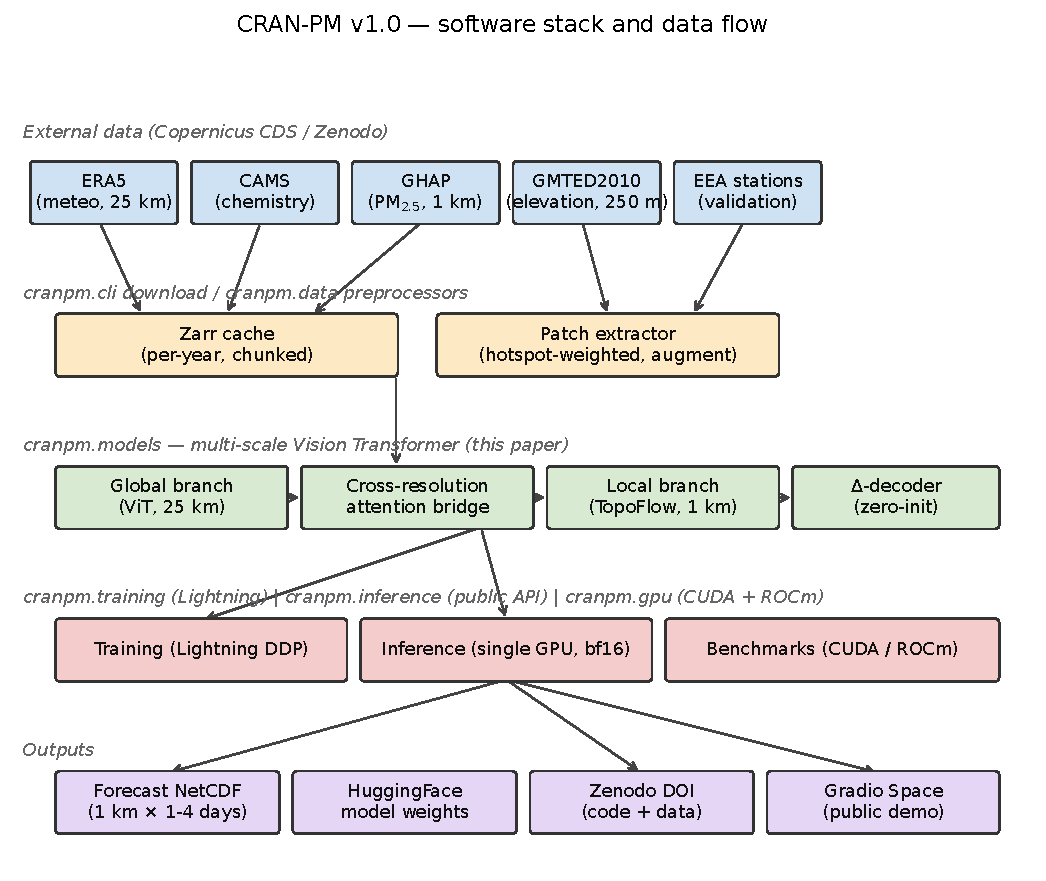
\includegraphics[width=\textwidth]{figures/fig_software_stack.pdf}
  \caption{\textbf{CRAN-PM v1.0 software stack.}
  External Copernicus and satellite data sources flow through
  configurable downloaders into a per-year zarr cache. The
  multi-scale Vision Transformer (Section~\ref{sec:model}) is
  trained with PyTorch Lightning DDP and served at inference time
  through a single-GPU public API. The GPU layer abstracts CUDA and
  ROCm. Outputs are forecast NetCDF files, archived model weights
  on HuggingFace, a citable Zenodo release and a Gradio web demo.}
  \label{fig:software_stack}
\end{figure}

\subsection{Package layout and public API}
\label{sec:soft:api}

The package follows the modern \texttt{src/} layout
\citep{copernicus_template}. The top-level package exposes a small
number of stable symbols:
\begin{verbatim}
from cranpm import CRANPMForecaster
model = CRANPMForecaster.from_pretrained(
    "AmmarKheder/cran-pm-europe-v3"
)
forecast = model.predict(
    era5=era5_dataset,        # xarray.Dataset
    cams=cams_dataset,        # xarray.Dataset
    elevation=elev_dataset,   # xarray.Dataset
    ghap_t0=ghap_dataset,     # xarray.Dataset (PM2.5 at t)
    lead_time=1,              # days
)
\end{verbatim}
Internally, \texttt{CRANPMForecaster} wraps the Lightning module,
a configuration object loaded from YAML and the GPU backend selector.
The same model is also exposed as a command-line tool:
\begin{verbatim}
cranpm forecast --date 2022-01-25 --region europe \
    --lead-time 1 --output forecast.nc
\end{verbatim}
\texttt{cranpm download era5} (and similar entry points for CAMS,
GHAP, GMTED2010, EEA) automate the corresponding Copernicus or USGS
downloads, resuming on partial failures.

Configuration is split between (i)~runtime paths via environment
variables (\texttt{CRANPM\_DATA\_ROOT}, \texttt{CRANPM\_CACHE\_DIR},
\texttt{CRANPM\_HF\_TOKEN}) and (ii)~scientific hyperparameters via
YAML files (\texttt{configs/europe\_multiscale.yaml}). This split
follows the practice common in operational atmospheric models where
file-system layout differs across compute centres but model physics
is portable.

\subsection{Data pipeline}
\label{sec:soft:data}

Inputs are stored as zarr \citep{miles2020zarr} arrays. Each
year-variable combination is one zarr group with chunking aligned
to the model's tile size ($512 \times 512$ for the local branch,
$168 \times 280$ for the global branch). Compression is
\texttt{Blosc(cname=zstd, clevel=3, shuffle=2)}. Downstream tile
extraction is performed by \texttt{cranpm.data.PatchExtractor},
which supports hot-spot weighted sampling (oversampling pixels with
historically high PM\textsubscript{2.5} concentrations to balance
the loss across the urban/rural distribution) and random
horizontal/vertical flips for augmentation.

Out-of-memory issues at high resolution are handled by streaming
tiles from zarr through PyTorch \texttt{DataLoader} workers; the
GHAP dataset alone is roughly 250\,GB per year and never fully
fits in RAM. Normalisation statistics for ERA5 and CAMS are stored
as Python constants in \texttt{cranpm.data.europe\_dataset} and
mirror the values used during training.

\subsection{GPU backend abstraction}
\label{sec:soft:gpu}

The package supports both NVIDIA CUDA and AMD ROCm in a single
codebase. Three engineering choices made this practical:
\begin{enumerate}
\item \textbf{F.unfold + nn.Linear in place of nn.Conv2d for patch
embeddings.} On AMD MI250X with ROCm 6.0.3, the MIOpen
implementation of \texttt{nn.Conv2d} for the patch embedding
($\text{kernel}=8$, $\text{stride}=8$, 65 input channels) produces
numerically diverging outputs in distributed training (peak
absolute error vs.\ a manual matmul reference of order $10$).
Replacing it with the equivalent \texttt{F.unfold + nn.Linear}
routes the call through rocBLAS, which is bit-stable. The CUDA
path is unaffected.
\item \textbf{Pre-scaling the attention logits.} The standard
$(\mathbf{Q} \mathbf{K}^\top) / \sqrt{d_h}$ formulation overflows
\texttt{bf16} on long token sequences. Computing
$(\mathbf{Q} / \sqrt[4]{d_h}) \cdot (\mathbf{K} /
\sqrt[4]{d_h})^\top$ instead removes the overflow and matches
the original numerics to within $10^{-3}$ relative error.
\item \textbf{Node-local MIOpen cache.} On LUMI the per-node
\texttt{/tmp} is independent. We launch one rank per node with
\texttt{srun -{}-ntasks-per-node=1} to populate the MIOpen cache on
every node before the main DDP launch.
\end{enumerate}
These choices are documented as \texttt{KNOWN\_ISSUES.md} in the
repository so that downstream contributors maintain compatibility.

The \texttt{cranpm.gpu} subpackage contains:
\texttt{infer\_single} (single-GPU inference with a configurable
precision), \texttt{train\_distributed} (DDP launcher portable
beyond LUMI) and \texttt{bench} (a reproducible benchmarking
harness, see Section~\ref{sec:perf}).

\subsection{Reproducibility infrastructure}
\label{sec:soft:repro}

The package ships with three layers of reproducibility tooling.

\paragraph{Pinned environments.}
A pinned dependency set gives an exact reproduction of the runtime
environment. A reproducible CPU/CUDA image
(\texttt{ghcr.io/ammarkheder/cran-pm:v1.0.0}) is built from
\texttt{docker/Dockerfile} and published automatically to the GitHub
Container Registry by a release workflow, providing a hermetic runtime
including system-level dependencies. Training on LUMI's AMD MI250X
partition uses the ROCm~6.0.3 stack through Singularity, documented in
the repository.

\paragraph{Continuous integration.}
GitHub Actions runs the unit and integration test suite on Python
3.10, 3.11 and 3.12 for every commit on \texttt{main} and every
pull request. The integration tests use a tiny synthetic dataset to
exercise the full forward and backward passes within a 5-minute
budget, ensuring that breaking changes are caught early.

\paragraph{Deterministic workflows.}
Training and evaluation seed Python, NumPy and PyTorch. The
checkpoint loader stores the configuration alongside the weights so
that a reload always reconstructs the same model topology.
The \texttt{cranpm reproduce} CLI regenerates each figure or table
from deposited intermediate outputs, e.g.
\texttt{cranpm reproduce -{}-figure fig\_method\_comparison}.

\subsection{Distribution surfaces}

The same model is distributed across three surfaces, each with a
distinct audience.
\begin{itemize}
\item \textbf{HuggingFace Hub} (\texttt{AmmarKheder/cran-pm-europe-v3})
serves the pre-trained weights as safetensors with an automatically
generated model card.
\item \textbf{HuggingFace Spaces} hosts a Gradio demo that runs
forecasts in the browser for users without GPU access. It targets
journalists and policy stakeholders.
\item \textbf{Zenodo} archives the source code release for citation
purposes (DOI \texttt{10.5281/zenodo.XXXXXXX}). The same DOI is
attached to the GitHub release, ensuring long-term retrievability.
\end{itemize}
